{
\newcommand\myrect[5]{\draw (#1,#2) rectangle ({#1+#3},{#2+#4}) node[pos=0.5] {#5} ; }

\begin{figure}
  \centering
  \begin{subfigure}[t]{0.24\textwidth}
        \centering
        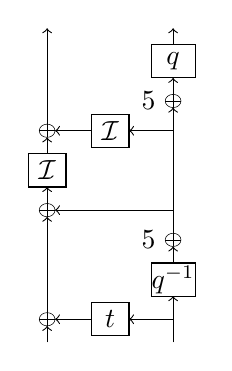
\begin{tikzpicture}[xscale=0.8, yscale=-0.42]
            \draw [->] (0,0) -- (0,-0.5);
            \draw [very thin] (0,-0.7) ellipse (0.125 and 0.2);
            \draw [very thin] (0,-0.9) -- (0,-0.5);
            \draw [very thin] (-0.125,-0.7) -- (0.125,-0.7);
            \draw (2,0) -- (2,-0.7);
            \draw [->] (2,-0.7) -- (1.3,-0.7);
            \draw (0.7,-1.2) rectangle (1.3,-0.2) node[pos=0.5] {$t$};
            \draw [->] (0.7,-0.7) -- (0.125,-0.7);
            \draw [->] (2,-0.7) -- (2,-1.4);
            \draw (1.65,-2.4) rectangle (2.35,-1.4) node[pos=0.5] {$q^{-1}$};
            \draw [->] (2,-2.4) -- (2,-2.9);
            \draw [very thin] (2,-3.1) ellipse (0.125 and 0.2);
            \draw [very thin] (2,-3.3) -- (2,-2.9);
            \draw [very thin] (1.875,-3.1) -- (2.125,-3.1);
            \draw (1.875,-3.1) node[anchor=east] {5};
            \draw [->] (0,-0.9) -- (0,-3.8);
            \draw [very thin] (0,-4) ellipse (0.125 and 0.2);
            \draw [very thin] (0,-4.2) -- (0,-3.8);
            \draw [very thin] (-0.125,-4) -- (0.125,-4);
            \draw (2,-3.3) -- (2,-4);
            \draw [->] (2,-4) -- (0.125,-4);
            \draw [->] (0,-4.2) -- (0,-4.7);
            \draw (-0.3,-5.7) rectangle (0.3,-4.7) node[pos=0.5] {$\mathcal{I}$};
            \draw [->] (0,-5.7) -- (0,-6.2);
            \draw [very thin] (0,-6.4) ellipse (0.125 and 0.2);
            \draw [very thin] (0,-6.6) -- (0,-6.2);
            \draw [very thin] (-0.125,-6.4) -- (0.125,-6.4);
            \draw (2,-4) -- (2,-6.4);
            \draw [->] (2,-6.4) -- (1.3,-6.4);
            \draw (0.7,-6.9) rectangle (1.3,-5.9) node[pos=0.5] {$\mathcal{I}$};
            \draw [->] (0.7,-6.4) -- (0.125,-6.4);
            \draw [->] (2,-6.4) -- (2,-7.1);
            \draw [very thin] (2,-7.3) ellipse (0.125 and 0.2);
            \draw [very thin] (2,-7.5) -- (2,-7.1);
            \draw [very thin] (1.875,-7.3) -- (2.125,-7.3);
            \draw (1.875,-7.3) node[anchor=east] {5};
            \draw [->] (2,-7.5) -- (2,-8);
            \draw (1.65,-9) rectangle (2.35,-8) node[pos=0.5] {$q$};
            \draw [->] (0,-6.6) -- (0,-9.5);
            \draw [->] (2,-9) -- (2,-9.5);
        \end{tikzpicture}
    \FigDef{simplify-T-linear-a}{}
  \end{subfigure}
  \hspace{0.3cm}
  \begin{subfigure}[t]{0.32\textwidth}
    \centering
      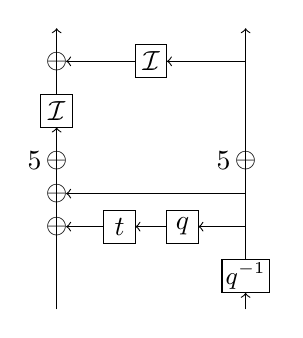
\begin{tikzpicture}[xscale=0.8, yscale=-0.42]
    	% right parallel, q
    	\draw [->] (2,3.5) -- (2,3);
    	\myrect{1.625}{2}{0.75}{1}{\small $q^{-1}$}
    	\draw [->] (2,2) -- (2,-5);
    	%\myrect{1.625}{-6.5}{0.75}{1}{\small $q^{\color{white}1}$}	
    	%\draw [->] (2,-6.5) -- (2,-7.5);
    
        % left bot to Inv
        \draw [->] (-1,3.5) -- (-1,-2);
    	% left Inv
    	\myrect{-1.25}{-3}{0.5}{1}{$\mathcal{I}$}
    	% I to p^{-1}
    	\draw [->] (-1,-3) -- (-1,-5);
    	% p^{-1}
    	%\myrect{-1.375}{-6.5}{0.75}{1}{\small $p^{-1}$}
    	% p^-1 to top
    	%\draw [->] (-1.0,-6.5) -- (-1.0,-7.5);
    
    	% right to q, t, xor
    	\draw [->] (2,1) -- (1.25,1);
    	\myrect{0.75}{0.5}{0.5}{1}{$q$}
    	\myrect{-0.25}{0.5}{0.5}{1}{$t$}
    	\draw [->] (0.75,1) -- (0.25,1);
    	\draw [->] (-0.25,1) -- (-0.85,1);
    	\draw (-1,1) node[inner sep=0]{$\oplus$} ;
    	
    	% right to xor
    	\draw [->] (2,0) -- (-0.85,0);
    	\draw (-1,0) node[inner sep=0]{$\oplus$} ;
    
    	% xor 5 on left
    	\draw (-1,-1) node[inner sep=0]{$\oplus$} ;
     	\draw (-1.35,-1) node[inner sep=0]{5} ;	
    
    	% xor 5 on right
    	\draw (2,-1) node[inner sep=0]{$\oplus$} ;
     	\draw (1.65,-1) node[inner sep=0]{5} ;	
    
    	% right to inv to xor
    	\draw [->] (2,-4) -- (0.75,-4);
    	\myrect{0.25}{-4.5}{0.5}{1}{$\mathcal{I}$}
    	\draw [->] (0.25,-4) -- (-0.85,-4);
    	\draw (-1,-4) node[inner sep=0]{$\oplus$} ;
    
    	% right xor 5 before q
    	%\draw (2,-4.75) node[inner sep=0]{$\oplus$};
     	%\draw (1.65,-4.75) node[inner sep=0]{5};	
    
    	% dots
    	%\draw [dotted] (-1.5,-0.5) rectangle (2.5,1.75);
      \end{tikzpicture}
    \FigDef{simplify-T-linear-b}{}
    %Moving $\mapsto q^{-1}(x+\elmt{2}{})$ around.
  \end{subfigure}
  \hspace{0.3cm}
  \begin{subfigure}[t]{0.32\textwidth}
    \centering
       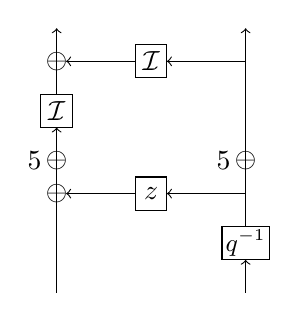
\begin{tikzpicture}[xscale=0.8, yscale=-0.42]
    	% right parallel, q
    	\draw [->] (2,3) -- (2,2);
    	\myrect{1.625}{1}{0.75}{1}{\small $q^{-1}$}
    	\draw [->] (2,1) -- (2,-5);
    	%\draw (2,-5) node[inner sep=0]{$\oplus$};
     	%\draw (1.65,-5) node[inner sep=0]{5};	
    	%\myrect{1.625}{-7}{0.75}{1}{\small $q^{\color{white}1}$}	
    	%\draw [->] (2,-7) -- (2,-8);
    
        % left bot to Inv
        \draw [->] (-1,3) -- (-1,-2);
    	% left Inv
    	\myrect{-1.25}{-3}{0.5}{1}{$\mathcal{I}$}
    	% I to p^{-1}
    	\draw [->] (-1,-3) -- (-1,-5);
    	% p^{-1}
    	%\myrect{-1.375}{-7}{0.75}{1}{\small $p^{-1}$}
    	% p^-1 to top
    	%\draw [->] (-1.0,-7) -- (-1.0,-8);
    
    	% right to [z] to xor
    	\draw [->] (2,0) -- (0.75,0);
    	\myrect{0.25}{-0.5}{0.5}{1}{$z$}
    	\draw [->] (0.25,0) -- (-0.85,0);
    	\draw (-1,0) node[inner sep=0]{$\oplus$} ;
    
    	% xor 5 on left
    	\draw (-1,-1) node[inner sep=0]{$\oplus$} ;
     	\draw (-1.35,-1) node[inner sep=0]{5} ;	
    
    	% xor 5 on right
    	\draw (2,-1) node[inner sep=0]{$\oplus$} ;
     	\draw (1.65,-1) node[inner sep=0]{5} ;	
    
    	% right to inv to xor
    	\draw [->] (2,-4) -- (0.75,-4);
    	\myrect{0.25}{-4.5}{0.5}{1}{$\mathcal{I}$}
    	\draw [->] (0.25,-4) -- (-0.85,-4);
    	\draw (-1,-4) node[inner sep=0]{$\oplus$} ;
    
    	% dots
    	%\draw [dashed] (-1.5,-7.5) rectangle (2.5,-4.6);
    	%\draw [dashed] (-1.5,-1.5) rectangle (2.5,2.5);
      \end{tikzpicture}
    \FigDef{simplify-T-linear-c}{}
    %Merging Feistel functions.
  \end{subfigure}
  \FigDef{simplify-t-linear}{Merging affine mappings in~the~decomposition~of~$T^{-1}$.}
\end{figure}

}